\subsection{Grokking for $K$-Wise Modular Addition}
\label{sec:subtask4}
In this task, we investigate the grokking phenomenon of $K$-wise modular addition. Due to the limitation of GPU memory, we only perform experiments on $2\leq K\leq 5$, and $p=31$. Specifically, we attempt to discover grokking phenomenon by adjusting training data fraction $\alpha$, and use techniques such as weight decay and dropout to lower down the scale of training data as much as possible. We use the transformer model which has the default parameters as shown in \cref{sec:subtask1}.

The minimal training steps required for memorization and generalization on different $\alpha$ is plotted in \cref{fig:grok_of_K=2_3}, for $K = 2, 3$ respectively. 
Comparing \cref{fig:grok_of_K=2} with \cref{fig:grok_of_K=3}, we discover that when $K=3$, generalization could happen at a smaller $\alpha$ than when $K=2$, but the gap between memorization and generalization is not as obvious as when $K=2$.    
\begin{figure}[!ht]
	\centering
	\begin{subfigure}{0.45\textwidth}
		\centering
		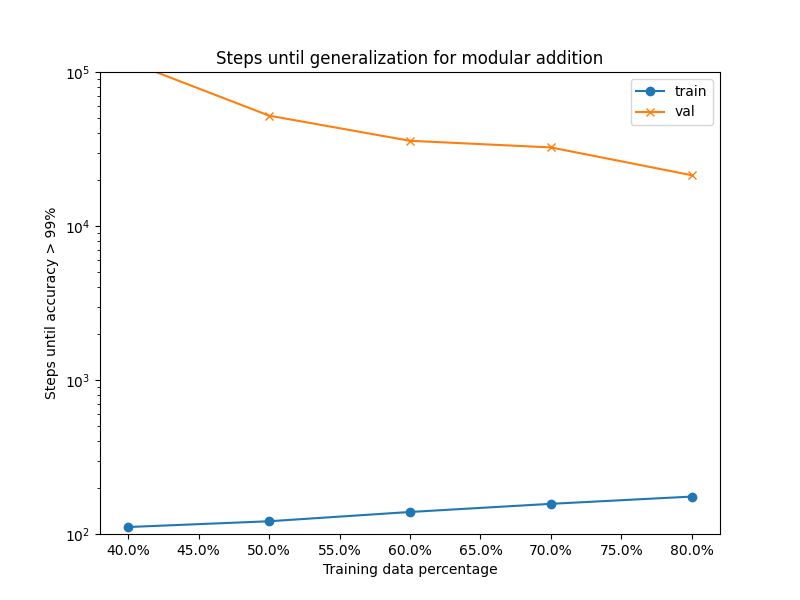
\includegraphics[width=\linewidth]{fig/Transformer_p=31/K=2/Transformer_alpha.png}
		\caption{Grokking phenomenon for $K=2$}
		\label{fig:grok_of_K=2}
	\end{subfigure}
	%\hfill
	\begin{subfigure}{0.45\textwidth}
		\centering
		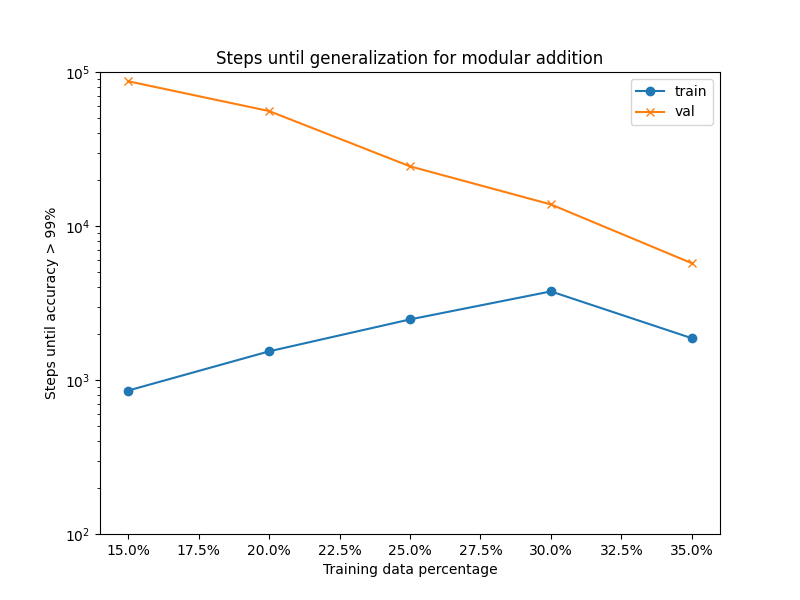
\includegraphics[width=\linewidth]{fig/Transformer_p=31/K=3/Transformer_alpha.png}
		\caption{Grokking phenomenon for $K=3$}
		\label{fig:grok_of_K=3}
	\end{subfigure}
	
	\caption{Grokking phenomenon for different $K$ and $\alpha$}
	\label{fig:grok_of_K=2_3}
\end{figure}
 
This above conclusion is also applied for $K=4$, but the grokking phenomenon is harder to discover. \cref{fig:K=4} illustrates the behaviors for $K=4$ with small variance $\alpha$. \cref{fig:alpha=9.0,fig:alpha=9.1} show that
generalization would happen before the training accuracy reaches $60\%$, and \cref{fig:alpha=9.2} shows that it is also possible that grokking would not happen with a small disturbance to $\alpha$. Besides, we do not find grokking phenomenon within $10^5$ steps when $\alpha\leq 8\%$.

In summary, the experiments imply that for a larger $K$, the model has better generalization performance, which could occur even for a small training data fraction.
Nevertheless, the grokking phenomenon becomes less apparent.
We provide an explanation of this in \cref{subsec:explain_by_regimes}.

\begin{figure}[!ht]
	\centering
	\begin{subfigure}{0.3\textwidth}
		\centering
		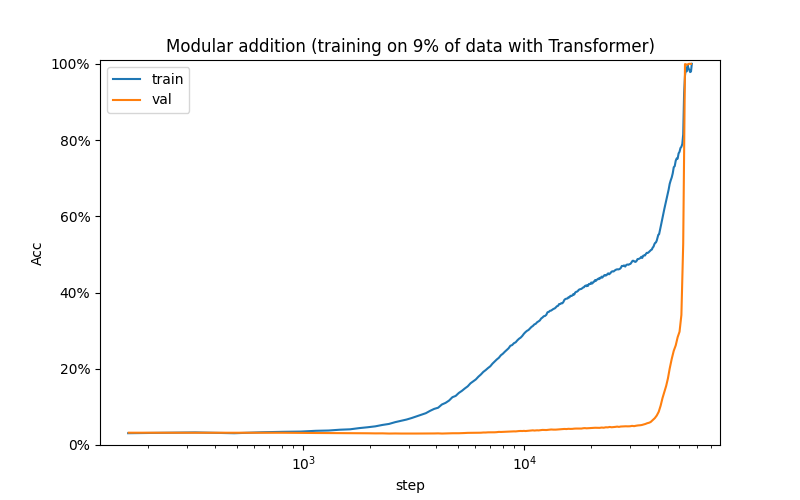
\includegraphics[width=\linewidth]{fig/Transformer_p=31/K=4/dropout=0.1,wd=0.1/alpha=9.0_dropout=0.1_wd=0.1/addition_9.0_Transformer_step.png}
		\caption{$\alpha=9.0\%$}
		\label{fig:alpha=9.0}
	\end{subfigure}
	%\hfill
		\begin{subfigure}{0.3\textwidth}
		\centering
		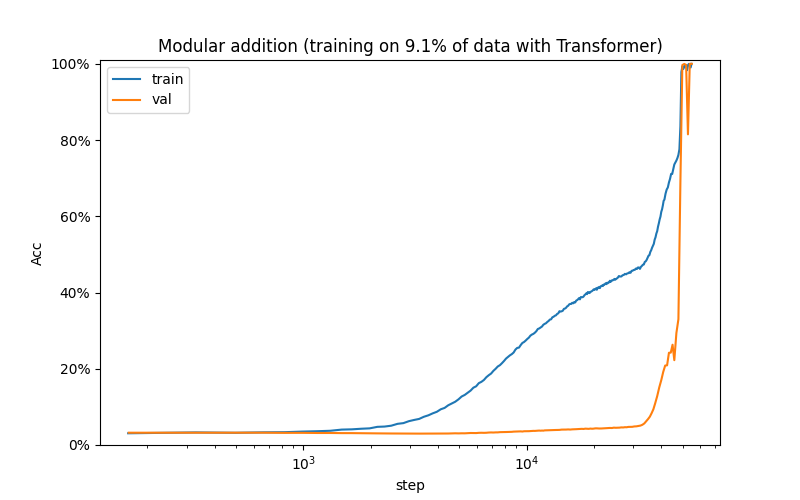
\includegraphics[width=\linewidth]{fig/Transformer_p=31/K=4/dropout=0.1,wd=0.1/alpha=9.1_dropout=0.1_wd=0.1/addition_9.1_Transformer_step.png}
		\caption{$\alpha=9.1\%$}
		\label{fig:alpha=9.1}
	\end{subfigure}
	%\hfill
	\begin{subfigure}{0.3\textwidth}
		\centering
		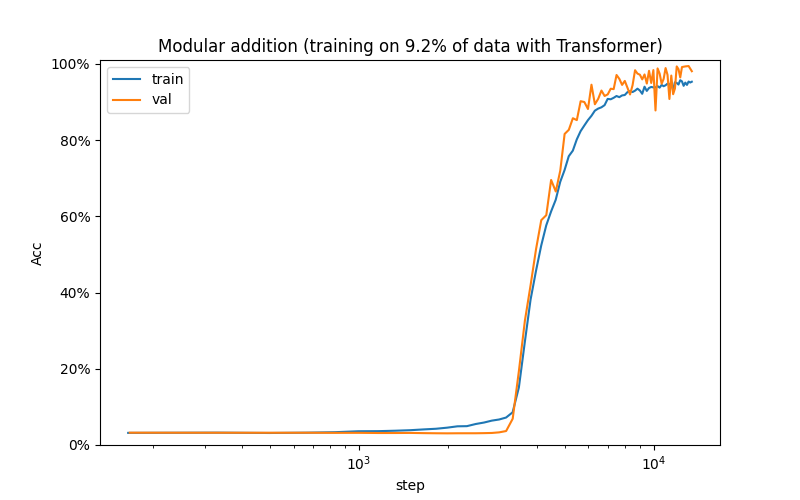
\includegraphics[width=\linewidth]{fig/Transformer_p=31/K=4/dropout=0.1,wd=0.1/alpha=9.2_dropout=0.1_wd=0.1/addition_9.2_Transformer_step.png}
		\caption{$\alpha=9.2\%$}
		\label{fig:alpha=9.2}
	\end{subfigure}
	\caption{Grokking phenomenon for $K=4$ with small variance $\alpha$}
	\label{fig:K=4}
\end{figure}

In addition, as \cref{fig:different_weight_decay_and_dropout} illustrates, we find that with proper adjustment to weight decay and dropout, the model could generalize with fewer training data, but sacrifice training stability.

\begin{figure}[!ht]
	\centering
	\begin{subfigure}{0.3\textwidth}
		\centering
		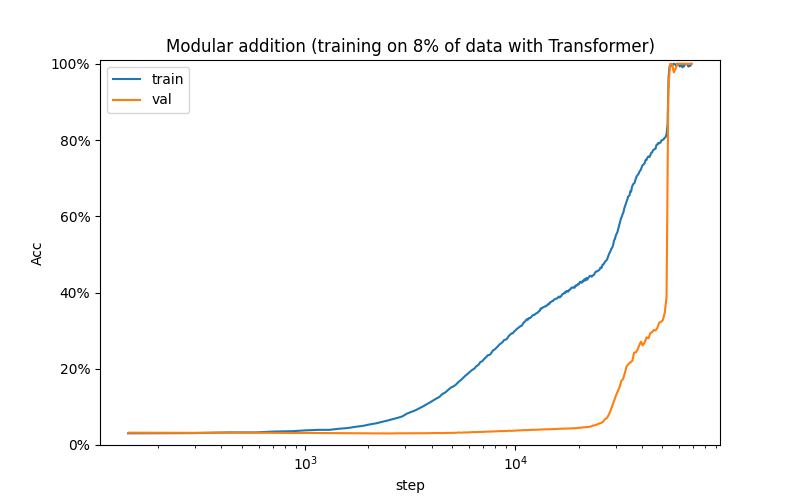
\includegraphics[width=\linewidth]{fig/Transformer_p=31/K=4/dropout=0.2,wd=0.1/alpha=8_dropout=0.2_wd=0.1/addition_8.0_Transformer_step.png}
		\caption{%
			\begin{tabular}{l}
				$\alpha = 8.0\%$ \\ 
				weight decay = 0.1 \\ 
				dropout = 0.2%
			\end{tabular}
		}
		\label{fig:alpha=8.0_wd=0.2_dp=0.1}
	\end{subfigure}
	%\hfill
	\begin{subfigure}{0.3\textwidth}
		\centering
		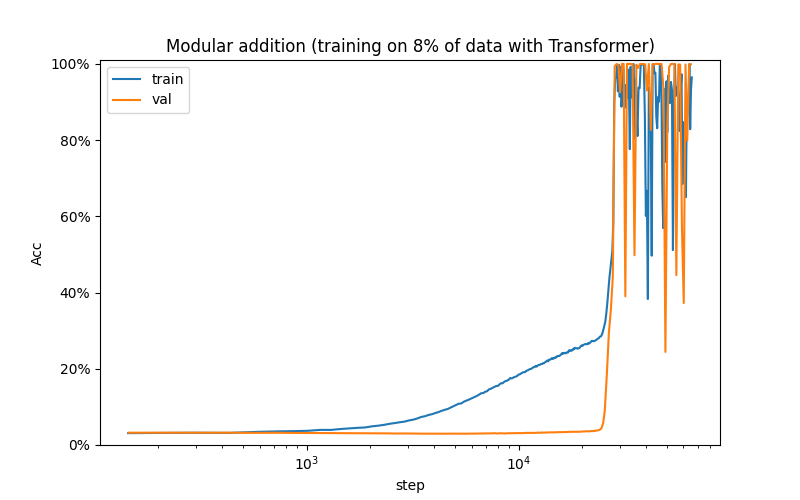
\includegraphics[width=\linewidth]{fig/Transformer_p=31/K=4/dropout=0.3,wd=0.2/alpha=8_dropout=0.3_wd=0.2/addition_8.0_Transformer_step.png}
				\caption{%
			\begin{tabular}{l}
				$\alpha = 8.0\%$ \\ 
				weight decay = 0.2 \\ 
				dropout = 0.3%
			\end{tabular}
		}
		\label{fig:alpha=8.0_wd=0.3_dp=0.2}
	\end{subfigure}
	%\hfill
	\begin{subfigure}{0.3\textwidth}
		\centering
		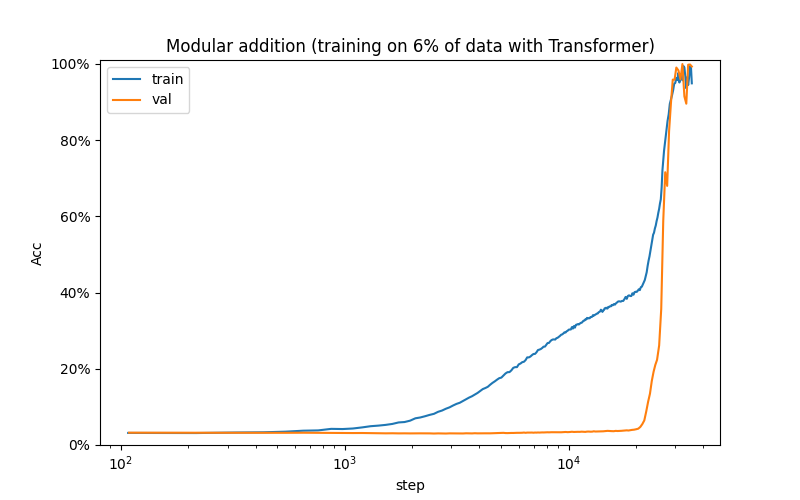
\includegraphics[width=\linewidth]{fig/Transformer_p=31/K=4/dropout=0.3,wd=0.2/alpha=6_dropout=0.3_wd=0.2/addition_6.0_Transformer_step.png}
				\caption{%
			\begin{tabular}{l}
				$\alpha = 6.0\%$ \\ 
				weight decay = 0.2 \\ 
				dropout = 0.3%
			\end{tabular}
		}
		\label{fig:alpha=6.0_wd=0.3_dp=0.2}
	\end{subfigure}
	\caption{Grokking phenomenon for $K=4$ with different weight decay and dropout}
	\label{fig:different_weight_decay_and_dropout}
\end{figure}
%The part for K=5 is optional, if space is not enough, just delete it. 
We further investigate the situation when $K=5$. Since it has an amount of more than $2\times 10^7$ data, we could only let $\alpha\leq 0.5\%$\footnote{Validation dataset is also limited. The dataset has been split into a training set and a validation set in a ratio of 1:3.}. This greatly limits our model's generalization ability and \cref{fig:alpha=0.5 without modified data} suggests no sign of generalization within $10^5$ training steps. Then we try to modify the training dataset by adding all equations of $K=2,3$ to it. Surprisingly the model successfully generalizes within $10^5$ steps with no more than $0.1\%$ training data fraction (not include equations we added) as \cref{fig:alpha=0.1 with modified data} shows.\footnote{The training accuracy quickly raises to about $50\%$ because the added equations account about $50\%$ in the training set. It seems that the model quickly learns the case of $K=2, 3$.} This suggests that the modification to training set may be effective. We look forward to further study about this technique on the larger $K$. 
\begin{figure}[!ht]
	\centering
	\begin{subfigure}{0.45\textwidth}
		\centering
		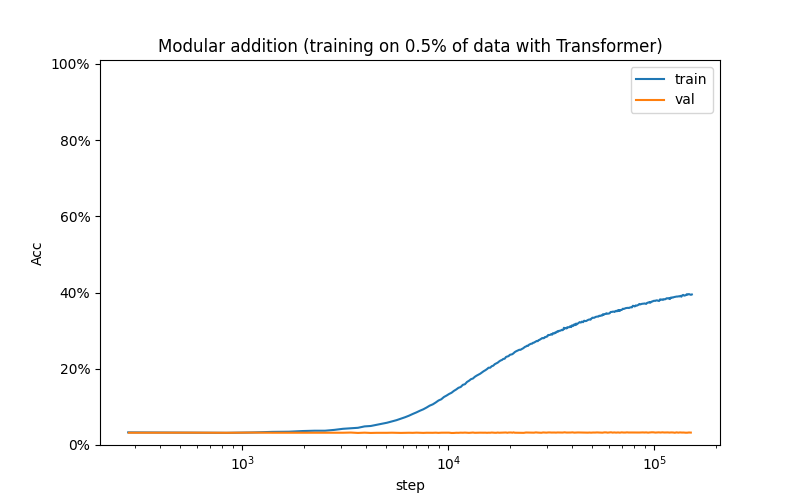
\includegraphics[width=\linewidth]{fig/Transformer_p=31/K=5/addition_0.5_Transformer_step.png}
		\caption{Train and val accuracy of $\alpha=0.5\%$ without modified data}
		\label{fig:alpha=0.5 without modified data}
	\end{subfigure}
	%\hfill
	\begin{subfigure}{0.45\textwidth}
		\centering
		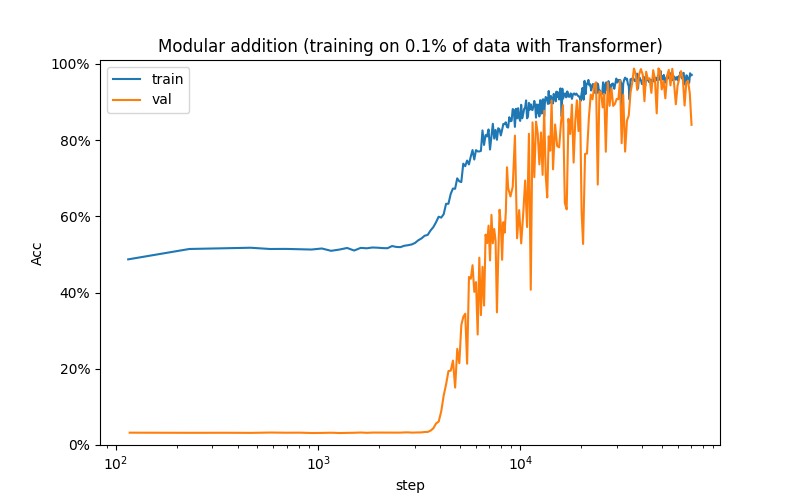
\includegraphics[width=\linewidth]{fig/Transformer_p=31/K=5/addition_0.1_Transformer_step.png}
		\caption{Train and val accuracy of $\alpha=0.1\%$ with modified data}
		\label{fig:alpha=0.1 with modified data}
	\end{subfigure}
	
	\caption{Grokking phenomenon for $K=5$}
	\label{fig:grok_of_K=5}
\end{figure}
